\chapter{光锥、测地线与施瓦茨席尔德视界}

视界问题始于狭义相对论中已经存在的一个区分。两个邻近事件可以沿类时、类空或类光方向分离。曲率并未废除这种分类。它使光锥成为局部对象，在每个事件处都不同，并使度规本身成为动力学量。一旦度规已知，自由下落粒子的运动就遵循与描述平直时空中自由相对论粒子相同的固有时原理。

我们将两次使用该原理。首先，它必须在弱场中重现牛顿运动。然后，它将被应用于施瓦茨席尔德度规，在那里，时间、径向距离和速度的含义会变得出乎意料地微妙。

\section{类时、类空与类光间隔}

在平直时空中，取\(c=1\)，固有时元为
\begin{equation}
d\tau^2=dt^2-dx^2-dy^2-dz^2.
\label{eq:l5-minkowski-proper-time}
\end{equation}
当非相对论近似接近时，恢复\(c\)是有用的：
\begin{equation}
d\tau^2
=dt^2-\frac{dx^2+dy^2+dz^2}{c^2}.
\label{eq:l5-minkowski-c}
\end{equation}
记号\(d\tau^2\)并不保证右侧为正。其符号对位移进行分类：
\begin{align}
d\tau^2>0
&\quad\Longleftrightarrow\quad \text{time-like},\\
d\tau^2=0
&\quad\Longleftrightarrow\quad \text{light-like},\\
d\tau^2<0
&\quad\Longleftrightarrow\quad \text{space-like}.
\end{align}
对于类空间隔，方便的是定义正固有距离
\begin{equation}
ds^2=-d\tau^2
=dx^2+dy^2+dz^2-dt^2
\qquad(c=1).
\label{eq:l5-proper-distance}
\end{equation}

光锥组织了这三种可能性。其表面，而非其填充的内部，由类光方向组成。类时方向位于锥内，类空方向位于锥外。上半部分和下半部分分别代表未来光锥和过去光锥。

\begin{figure}[htbp]
\centering
\includegraphics[width=0.82\textwidth]{lecture_05_figure_02.png}
\caption{在黑板上汇集的固有时、固有距离与因果锥。光线占据锥面本身；内部为类时，外部为类空。}
\lectureframe{00:05:44}
\end{figure}

\begin{figure}[htbp]
\centering
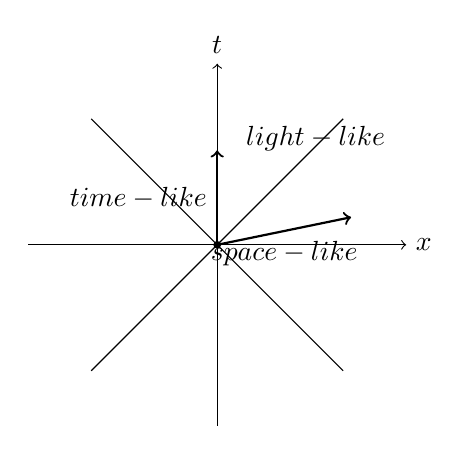
\begin{tikzpicture}[scale=1.0]
\draw[->] (0,-2.3) -- (0,2.3) node[above] {\(t\)};
\draw[->] (-2.4,0) -- (2.4,0) node[right] {\(x\)};
\draw (-1.6,1.6) -- (0,0) -- (1.6,1.6);
\draw (-1.6,-1.6) -- (0,0) -- (1.6,-1.6);
\fill (0,0) circle (1.4pt);
\draw[->,thick] (0,0) -- (0,1.2)
  node[midway,left] {\(\text{time-like}\)};
\draw[->,thick] (0,0) -- (1.7,0.35)
  node[midway,below] {\(\text{space-like}\)};
\node at (1.25,1.35) {\(\text{light-like}\)};
\end{tikzpicture}
\caption{二维时空截面中的因果分类。}
\end{figure}

这些间隔是可操作的。固有时是沿类时世界线携带的时钟所读出的量。固有距离是合适的量尺组在类空分离事件之间所测得的量。它们不仅仅是二次形式中符号的名称。

\section{洛伦兹号差与每个事件处的锥}

使用mostly-plus张量约定，平直度规的分量为
\begin{equation}
\eta_{\mu\nu}=\operatorname{diag}(-1,1,1,1),
\label{eq:l5-eta}
\end{equation}
以及
\begin{equation}
d\tau^2=-\eta_{\mu\nu}\,dx^\mu dx^\nu.
\label{eq:l5-proper-time-eta}
\end{equation}
所显示的矩阵是二阶张量在一个特别简单的基中的表达式。其不变特征是它的号差：一个负方向和三个正方向，
\begin{equation}
\operatorname{signature}(\eta)=(-,+,+,+).
\label{eq:l5-lorentz-signature}
\end{equation}
具有两个负号的度规将有两个时间方向。这样的号差可以在数学上研究，但它们并不描述这里所假设的时空。

在弯曲时空中，分量会变化：
\begin{equation}
g_{\mu\nu}=g_{\mu\nu}(x).
\label{eq:l5-position-metric}
\end{equation}
在每个事件处，度规仍必须具有洛伦兹号差。因此，每个事件都有自己的类时方向、类光边界和类空方向。坐标图可能显示锥从一点到另一点倾斜或压扁，但因果分类保持不变。

\begin{figure}[htbp]
\centering
\includegraphics[width=0.86\textwidth]{lecture_05_figure_03.png}
\caption{位置相关的度规\(g_{\mu\nu}(x)\)、因果标签以及局部光锥的草图。}
\lectureframe{00:09:41}
\end{figure}

\begin{figure}[htbp]
\centering
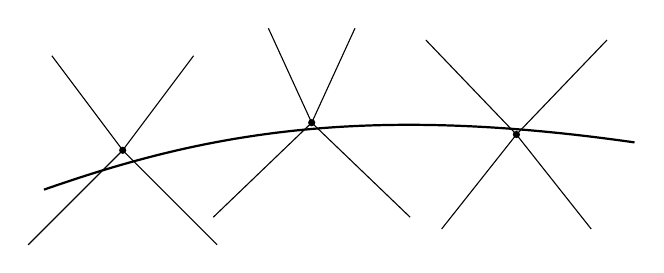
\begin{tikzpicture}[scale=1.0]
\draw[thick] (-4,-0.5) .. controls (-2,0.2) and (0,0.6) .. (3.5,0.1);
\foreach \x/\y/\a/\b in {-3/0/0.9/1.2, -0.6/0.35/0.55/1.25,
                          2.0/0.2/1.15/0.95} {
  \fill (\x,\y) circle (1.3pt);
  \draw (\x,\y) -- ++(-\a,1.2);
  \draw (\x,\y) -- ++(\a,1.2);
  \draw (\x,\y) -- ++(-\b,-1.2);
  \draw (\x,\y) -- ++(\b,-1.2);
}
\end{tikzpicture}
\caption{相邻的局部锥。它们的坐标形状可以改变，而不改变哪些矢量是类时、类光或类空。}
\end{figure}

\begin{classroomqa}
\audiencequestion{单个负本征值是否选择了一个唯一的时间方向？}
\lecturerresponse{使所显示矩阵对角化的基有一个负的基方向，但这并不选择优先的观测者或唯一的物理箭头。洛伦兹变换将时间坐标与空间坐标混合，而锥内的每个矢量都是类时的。不变的对象是锥连同one-minus, three-plus号差，而不是一个特殊的类时矢量。
\lecturetimestamp{00:12:17--00:17:24}}
\end{classroomqa}

\begin{classroomqa}
\audiencequestion{为什么局部锥的两幅图可以有不同的形状？}
\lecturerresponse{坐标可以改变图形。例如，将\(x\)替换为重新标度的坐标会改变赋予光线的数值斜率，从而使锥显得更窄或更宽。更一般的坐标可以使其倾斜。所表示的是同一事件和同样的因果关系。在弯曲时空中，不同事件处的锥也属于不同的切空间，因此它们的比较需要度规和输运规则。
\lecturetimestamp{00:13:37--00:15:59}}
\end{classroomqa}

\section{作为变分问题的测地线}

自由运动的粒子沿时空测地线运动。用仿射参数\(\lambda\)写成微分形式，
\begin{equation}
\frac{d^2x^\mu}{d\lambda^2}
+\Gamma^\mu{}_{\rho\sigma}
\frac{dx^\rho}{d\lambda}
\frac{dx^\sigma}{d\lambda}=0.
\label{eq:l5-geodesic}
\end{equation}
联络告诉切矢量如何在粒子运动时保持与自身平行。

还有第二种表述，用它计算往往更容易。在具有度规\(g_{mn}\)的黎曼空间中，曲线的长度为
\begin{equation}
s=\int ds
=\int\sqrt{g_{mn}\,dx^m dx^n}.
\label{eq:l5-spatial-length}
\end{equation}
测地线使这一长度在端点固定、路径作微小变动时取驻值。该积分就是沿曲线的无穷小长度之和，其Euler--Lagrange方程是一个二阶微分方程，形式类似于力的定律。

对于类时世界线，空间长度由固有时取代：
\begin{equation}
\tau
=\int\sqrt{-g_{\mu\nu}\,dx^\mu dx^\nu}.
\label{eq:l5-proper-time-functional}
\end{equation}
类时测地线使\(\tau\)取驻值，并且在共轭点出现之前，对于邻近的自由下落路径，它取局部极大值。乘以\(-m\)得到粒子作用量
\begin{equation}
A=-m\tau
=-m\int\sqrt{-g_{\mu\nu}\,dx^\mu dx^\nu}.
\label{eq:l5-particle-action}
\end{equation}
因此同一条路径在局部使\(A=-m\tau\)取极小值。取驻值的固有时与所选作用量的符号之间的区别，消除了表面上极小与极大的歧义。

\section{从固有时到普通拉格朗日量}

\eqref{eq:l5-particle-action}中的作用量是几何的，但可以写成力学中熟悉的常用形式。用坐标\(t\)参数化世界线，将每个微分除以\(dt\)，并把剩余的因子\(dt\)提到平方根之外：
\begin{align}
A
&=-m\int\sqrt{-g_{\mu\nu}(x)\,dx^\mu dx^\nu}\\
&=-m\int
\sqrt{-g_{\mu\nu}(x)
\frac{dx^\mu}{dt}\frac{dx^\nu}{dt}}\,dt.
\label{eq:l5-action-t}
\end{align}
对于时间分量\(dt/dt=1\)；空间分量就是普通的坐标速度。因此我们可以写出
\begin{equation}
\begin{aligned}
A&=\int L\,dt,\\
L&=-m\sqrt{-g_{\mu\nu}(x)\dot x^\mu\dot x^\nu},\\
\dot x^\mu&=\frac{dx^\mu}{dt}.
\end{aligned}
\label{eq:l5-relativistic-lagrangian}
\end{equation}

\begin{figure}[htbp]
\centering
\includegraphics[width=0.88\textwidth]{lecture_05_figure_05.png}
\caption{世界线作用量被转换为传统形式\(A=\int L\,dt\)。}
\lectureframe{00:27:00}
\end{figure}

\begin{figure}[htbp]
\centering
\includegraphics[width=0.88\textwidth]{lecture_05_figure_06.png}
\caption{稍后的板书状态，其中相对论性拉格朗日量已被分离出来。}
\lectureframe{00:28:59}
\end{figure}

\begin{classroomqa}
\audiencequestion{这个作用量中的时空指标应该是希腊字母吗？}
\lecturerresponse{是的。希腊指标遍历时间和所有空间坐标。当这种区分有用时，拉丁指标可以保留给空间坐标。
\lecturetimestamp{00:25:53--00:26:03}}
\end{classroomqa}

\begin{classroomqa}
\audiencequestion{为什么这个平方根表达式被称为拉格朗日量？}
\lecturerresponse{在作用量被写成\(A=\int L\,dt\)之后，被积函数就是拉格朗日量。这不仅仅是一个定义：对该被积函数作变分给出Euler--Lagrange方程
\[
\frac{d}{dt}
\left(\frac{\partial L}{\partial\dot x^\mu}\right)
=\frac{\partial L}{\partial x^\mu},
\]
在参数化被一致处理后，它们等价于测地线方程。
\lecturetimestamp{00:28:36--00:29:02}}
\end{classroomqa}

对于有质量粒子，世界线是类时的，因此平方根下的量为正。类空路径将描述超光速运动，而不是普通有质量粒子的轨迹。给定度规后，现在既可以通过计算Christoffel符号并使用\eqref{eq:l5-geodesic}来得到粒子的路径，也可以对\eqref{eq:l5-relativistic-lagrangian}应用Euler--Lagrange来得到。证明二者的等价性是一个有用的练习；作用量途径通常更短。

\section{牛顿极限}

考虑球对称源外部的弱静态引力场。从平直时空出发，允许\(dt^2\)的系数略微偏离1：
\begin{equation}
d\tau^2
=\left(1+\frac{2u(\mathbf{x})}{c^2}\right)dt^2
-\frac{d\mathbf{x}^2}{c^2},
\label{eq:l5-weak-metric}
\end{equation}
其中\(u\)将成为牛顿势。这个假设必须被检验，而不能仅仅被命名。

有量纲的粒子作用量为
\begin{equation}
A=-mc^2\int
\sqrt{1+\frac{2u}{c^2}
-\frac{\dot{\mathbf{x}}^{\,2}}{c^2}}\,dt.
\label{eq:l5-weak-action}
\end{equation}
\(u/c^2\)和\(\dot{\mathbf{x}}^{\,2}/c^2\)都很小。保留它们的一阶贡献，
\begin{equation}
\sqrt{1+\epsilon}
=1+\frac{\epsilon}{2}+O(\epsilon^2),
\qquad
\epsilon=\frac{2u-\dot{\mathbf{x}}^{\,2}}{c^2},
\end{equation}
给出
\begin{align}
L
&=-mc^2
\sqrt{1+\frac{2u-\dot{\mathbf{x}}^{\,2}}{c^2}}\\
&=-mc^2-mu+\frac{m}{2}\dot{\mathbf{x}}^{\,2}\\
&\quad+O\!\left(c^{-2}
 [u^2+u\dot{\mathbf{x}}^{\,2}+\dot{\mathbf{x}}^{\,4}]\right).
\label{eq:l5-newton-expansion}
\end{align}
常数静能项对运动方程没有影响。剩下的是
\begin{equation}
L_{\mathrm{nr}}
=\frac{m}{2}\dot{\mathbf{x}}^{\,2}-m u(\mathbf{x}),
\label{eq:l5-newton-lagrangian}
\end{equation}
因此
\begin{equation}
m\ddot{\mathbf{x}}=-m\boldsymbol{\nabla}u.
\label{eq:l5-newton-equation}
\end{equation}
试验质量被消去，这正是普遍自由下落所要求的。势能是\(m u\)，而加速度与\(m\)无关。

因此我们确定了领先阶的弱场关系
\begin{equation}
g_{00}=1+\frac{2u}{c^2}+O(c^{-4}).
\label{eq:l5-g00-newton}
\end{equation}
在球对称质量\(M\)外部，
\begin{equation}
u(r)=-\frac{GM}{r},
\qquad
g_{00}=1-\frac{2GM}{rc^2}+O(c^{-4}).
\label{eq:l5-g00-spherical}
\end{equation}
这确定了时间分量的第一阶修正。它尚未确定完整的强场度规。

\section{球坐标与第一个Schwarzschild猜测}

对于中心源，球坐标是自然的。本讲从赤道面而不是从极点量度\(\theta\)，因此其角向线元为
\begin{equation}
d\Omega^2=d\theta^2+\cos^2\theta\,d\phi^2.
\label{eq:l5-angular-metric}
\end{equation}
采用这一约定，
\begin{equation}
d\mathbf{x}^2=dr^2+r^2d\Omega^2.
\label{eq:l5-flat-spherical}
\end{equation}
没有任何物理内容依赖于选择这个类似纬度的\(\theta\)；使用更常见的极角会把\(\cos^2\theta\)替换为\(\sin^2\theta\)。

在保持空间度规平坦的同时插入牛顿时间系数，得到第一个猜测
\begin{equation}
\begin{aligned}
d\tau^2
&=\left(1-\frac{r_s}{r}\right)dt^2
-\frac{1}{c^2}\left(dr^2+r^2d\Omega^2\right),\\
r_s&=\frac{2GM}{c^2}.
\end{aligned}
\label{eq:l5-naive-schwarzschild}
\end{equation}
这不可能是精确答案。对于\(r<r_s\)，在固有时间约定下，\(dt^2\)的系数改变符号，而每个空间系数仍为负。度规将失去一时间和三空间的号差。

真空场方程给出了所需的径向系数：
\begin{equation}
\boxed{
d\tau^2
=\left(1-\frac{r_s}{r}\right)dt^2
-\frac{dr^2}{c^2\left(1-r_s/r\right)}
-\frac{r^2}{c^2}d\Omega^2.
}
\label{eq:l5-schwarzschild}
\end{equation}
这就是外史瓦西度规。当\(r\)经过\(r_s\)时，\(t\)和\(r\)的系数一起改变符号，从而保持洛伦兹号差。在史瓦西坐标中，径向坐标在内部变为类时，而坐标\(t\)变为类空。这种交换标志着坐标图在视界处的失效，而不是时空几何本身的局部失效。

\begin{classroomqa}
\audiencequestion{下落物体穿过视界需要多长时间？}
\lecturerresponse{用遥远观测者所使用的史瓦西坐标\(t\)来测量，穿越被推迟到无限时间。用下落物体时钟上的固有时间来测量，它发生在有限时间内。这两个时钟之间的区别正是视界谜题的核心。
\lecturetimestamp{00:54:45--00:55:35}}
\end{classroomqa}

\begin{classroomqa}
\audiencequestion{为什么要改变径向系数，而不是度规的其他部分？}
\lecturerresponse{度规必须保持洛伦兹号差，球对称性将径向方向与角向球面区分开来，而真空场方程精确地确定了倒数因子。仅号差就提示了该从哪里寻找；爱因斯坦方程给出了精确结果。
\lecturetimestamp{00:55:35--00:56:01}}
\end{classroomqa}

对于地球，\(r_s\)只有大约一厘米的量级，深处于物质体内部。外真空度规在那里不成立，因此地球没有史瓦西视界。在物质内部必须用内部解来替代它，并在表面与之匹配。

\begin{classroomqa}
\audiencequestion{如果\(t\)和\(r\)交换坐标角色，普通时钟会发生什么？}
\lecturerresponse{时钟继续沿着类时世界线测量固有时间。它并不知道所选的坐标已变得不便使用。一个规则的自由下落坐标系显示出光滑的局部几何，以及穿过视界的普通局部光传播。
\lecturetimestamp{00:56:35--00:57:50}}
\end{classroomqa}

\subsection{为什么径向修正没有出现在牛顿方程中}

精确度规在势的一阶就已经改变了径向系数：
\begin{equation}
\frac{1}{1-r_s/r}
=1+\frac{r_s}{r}
+O\!\left(\frac{r_s^2}{r^2}\right)
=1-\frac{2u}{c^2}+O(c^{-4}).
\label{eq:l5-radial-expansion}
\end{equation}
为什么在牛顿推导中忽略这一改变是合理的？在粒子作用量内部，它乘以\(\dot r^2/c^2\)。因此它的第一项修正正比于
\begin{equation}
\frac{u\,\dot r^2}{c^4},
\end{equation}
这超出了\eqref{eq:l5-newton-expansion}中所保留的阶。对于慢速运动的牛顿检验，径向修正是可忽略的，然而对于相对论运动以及在视界附近，它变得具有决定性。这是一个有用的警告：对一种近似来说太小的项，在另一种近似中可能控制着所关注的现象。

\section{史瓦西时间中的径向下落}

设\(c=1\)，首先研究径向运动。圆轨道也很重要，但它们需要角向项，因此推迟讨论。径向运动与其说是轨道，不如说是直接朝源坠落，并且它以最少的代数揭示了视界行为。

\begin{classroomqa}
\audiencequestion{径向速度中出现的是谁的时间？}
\lecturerresponse{下面的点表示对史瓦西坐标时间\(t\)求导，该时间被归一化为遥远静态观测者的时间。下落观测者的手表测量固有时间\(\tau\)。混淆两者会把一个坐标陈述变成错误的局部陈述。
\lecturetimestamp{01:04:03--01:04:47}}
\end{classroomqa}

对于\(d\Omega=0\)，定义
\begin{equation}
a(r)=1-\frac{r_s}{r}.
\label{eq:l5-a-def}
\end{equation}
径向度规和拉格朗日量为
\begin{align}
d\tau^2&=a\,dt^2-\frac{dr^2}{a},\\
L&=-m\sqrt{a-\frac{\dot r^2}{a}},
\qquad
\dot r=\frac{dr}{dt}.
\label{eq:l5-radial-lagrangian}
\end{align}
因为\(L\)没有显式的\(t\)依赖，其哈密顿量守恒。径向动量为
\begin{equation}
p_r=\frac{\partial L}{\partial\dot r}
=\frac{m\dot r}{a\sqrt{a-\dot r^2/a}},
\label{eq:l5-radial-momentum}
\end{equation}
并且
\begin{align}
H
&=p_r\dot r-L\\
&=\frac{ma}{\sqrt{a-\dot r^2/a}}
=E.
\label{eq:l5-radial-energy}
\end{align}
解出坐标速度得到
\begin{equation}
\boxed{
\dot r^2
=a^2\left(1-\frac{m^2}{E^2}a\right).
}
\label{eq:l5-radial-velocity}
\end{equation}
黑板上的计算检验了几个中间代数形式；方框中的表达式是一致的结果。

当\(r\)趋近\(r_s\)时，\(a(r)\)趋近于零，而括号中的因子趋近于一。因此
\begin{equation}
\frac{dr}{dt}
\sim -\left(1-\frac{r_s}{r}\right)
\longrightarrow 0
\qquad(r\longrightarrow r_s^+)
\label{eq:l5-infall-freeze}
\end{equation}
对于入射粒子。在史瓦西时间中，粒子似乎减速并冻结在视界外侧。

\begin{classroomqa}
\audiencequestion{\(dr/dt\)的值不断减小，是否意味着引力
变成了斥力？}
\lecturerresponse{不是。粒子并没有在局部被向外推。坐标\(t\)变得越来越不适合描述这一穿越，
因此每单位\(t\)的径向进展趋于零。沿自由下落世界线的固有加速度仍为零，
而视界是在有限固有时间内到达的。
\lecturetimestamp{01:14:18--01:16:38}}
\end{classroomqa}

事实上，在视界附近
\begin{equation}
\frac{dt}{dr}
\sim-\frac{1}{1-r_s/r}
=-\frac{r}{r-r_s}.
\end{equation}
其积分按对数发散。这证明了无限施瓦西时间的说法，
而并不意味着下落时钟上的读数为无限。

\section{径向光线}

光给出了同一计算的最简版本。对于径向零测地线，
\begin{equation}
d\tau^2
=a\,dt^2-\frac{dr^2}{a}=0.
\end{equation}
因此
\begin{equation}
\boxed{
\frac{dr}{dt}
=\pm a(r)
=\pm\left(1-\frac{r_s}{r}\right).
}
\label{eq:l5-radial-light}
\end{equation}
正号描述出射光线，负号描述入射光线。
两种坐标速度在视界处都趋于零。

\begin{classroomqa}
\audiencequestion{该公式在远离源处给出什么速度？}
\lecturerresponse{当\(r\)趋于无穷大时，\(a(r)\)趋于一，因此
\(dr/dt\)趋于\(\pm1\)，或者恢复单位后趋于\(\pm c\)。
\lecturetimestamp{01:21:01--01:21:29}}
\end{classroomqa}

广义相对论常常如此：原理只需几行，
而坐标和计算却变得复杂。方程
\eqref{eq:l5-radial-light}很简单，但解释它在\(r_s\)附近消失却需要小心。
它是坐标速度，而不是局部惯性观测者测得的速度。

\section{远处观测者看到什么}

\begin{classroomqa}
\audiencequestion{在视界附近发出的光能逃逸吗？那是
霍金辐射吗？}
\lecturerresponse{在视界外侧刚刚发出的经典出射光线
可以向外运动，但它的施瓦西坐标速度起初极其微小，信号要经过严重的延迟和
红移之后才能到达无穷远。视界上的光线在这些坐标中仍留在视界上；
视界内的光线无法逃逸。霍金辐射是一种与外部几何相关的量子场效应，
而不是从内部爬出来的经典光线，并且它不是由当前计算推导出来的。
\lecturetimestamp{01:22:08--01:24:28}}
\end{classroomqa}

\begin{classroomqa}
\audiencequestion{如果一个光子看起来几乎静止，它是否开始显得
有质量？}
\lecturerresponse{不是。自由下落的局部观测者总是测得
光子以\(c\)运动。只有坐标比值\(dr/dt\)趋于零。
质量、零性以及局部光速都不会因糟糕的坐标图而改变。
\lecturetimestamp{01:24:31--01:25:26}}
\end{classroomqa}

这里使用的施瓦西表达式是真空外部解。恒星、行星或坍缩云具有不同的内部度规，必须与之匹配。如果物质表面保持在\(r_s\)之外，正如地球以极大的余量所做的那样，那么外部坐标视界就位于真空公式能够穿过物质继续延拓的区域之外。如果天体坍缩到其施瓦西半径以内，视界就成为物理时空的一部分。

\begin{classroomqa}
\audiencequestion{如果外部观测者永远看不到物质穿越，黑洞又如何能够形成或增长？}
\lecturerresponse{这一前提把施瓦西时间当成了视界处的全局物理时钟。由此得出黑洞因此永远不能增长的结论听起来合理，但却是错误的。完整的回答需要规则的穿越视界坐标以及坍缩的全局因果几何；这一解决留待本课程的下一阶段。
\lecturetimestamp{01:27:57--01:29:36}}
\end{classroomqa}

\begin{classroomqa}
\audiencequestion{对于一辆朝视界下落的汽车，雷达测速枪会报告什么？}
\lecturerresponse{坐标速度随着汽车下落先增大，随后转折并减小趋于零。稍后发出的雷达脉冲仍能在视界外追上汽车，但往返所需时间越来越长。返回信号的红移越来越大，图像在\(r_s\)附近显得变慢并被压缩。这并不是驾驶员所经历情形的可靠局部图像；驾驶员在有限固有时间内穿越。
\lecturetimestamp{01:29:39--01:32:14}}
\end{classroomqa}

\begin{classroomqa}
\audiencequestion{光速只在狭义相对论中才是常数吗？}
\lecturerresponse{在广义相对论中，它在每一个局部惯性系中同样是常数。一个带着局部时钟和米尺下落的观测者测得附近光子以\(c\)运动。诸如\(dr/dt\)这样的坐标速度可以变化，因为\(r\)和\(t\)并不是同一个局部惯性实验室在整个时空上的读数。
\lecturetimestamp{01:32:20--01:34:20}}
\end{classroomqa}

\section{施瓦西计算之外的问题}

\begin{classroomqa}
\audiencequestion{把引力与其他力统一起来可能意味着什么？}
\lecturerresponse{一种几何上的可能性是用额外的紧致方向来扩充时空。高维度规的分量于是在四维中表现为规范场和标量场，而沿额外方向的动量则可以表现为一种荷。这是与Kaluza--Klein思想相关的一个结构性提示，而不是本次讲座中已完成的统一。
\lecturetimestamp{01:34:22--01:36:08}}
\end{classroomqa}

\begin{classroomqa}
\audiencequestion{不同的区域或宇宙可以有不同的度规号差吗？}
\lecturerresponse{经典广义相对论通常固定一个非退化的洛伦兹号差。要改变它，度规就必须经过一个退化位形，而标准的经典描述在那里失效。量子引力也许会迫使我们采用更宽广的语言，但在这里并不存在任何已确立的理论能预言物理上改变号差的区域。
\lecturetimestamp{01:36:08--01:38:08}}
\end{classroomqa}

\begin{classroomqa}
\audiencequestion{施瓦茨席尔德在第一次世界大战期间服役时，是如何找到这个解的？}
\lecturerresponse{课上所强调的一点既是历史性的，也是关乎人的：施瓦茨席尔德是一位天文学家，也是一位造诣极高的数学家，而在战时服役期间钻研爱因斯坦的新方程为他提供了一处精神上的避难所。
\lecturetimestamp{01:38:11--01:39:02}}
\end{classroomqa}

核心教训如今已经足够清晰，可以继续推进了。度规同时决定因果锥和自由运动。它的弱场时间分量包含牛顿势，而它的精确施瓦茨席尔德形式则在\(r=r_s\)处给出一个坐标视界。施瓦茨席尔德时间把穿越拉伸到无穷；下落观测者的固有时则不然。从全局上解决这一反差，并解释尽管远处的图像被冻结、黑洞究竟如何形成，就是下一个问题。
